%% ==============================
\chapter{\iflanguage{ngerman}{Ergebnisse}{Results}}
\label{sec:results}
%% ==============================





Diese Kapitel beschäftigt sich mit den Ergebnissen und der Evaluation dieser Bachelorarbeit. Die Ergebnisse der Visualisierung sind in mehreren Abbildungen zu sehen. Die Evaluation teilt sich folgendermaßen auf. Als erstes werden die Ergebnisse der Visualisierung des Ventrikelsystems gezeigt und evaluiert. Die Auswertung wurde in Form eines Interviews mit einem Arzt durchgeführt. Danach wird eine Nutzerstudie vorgestellt, die die Usability des Systems testet. Als letztes wird die Berechnungszeit der Implementierung besprochen.



In dieser Arbeit wurden hauptsächlich Volumen mit einer Auflösung von 256x101x256 Pixeln verwendet, da gut erkennbare Ergebnisse damit erzielt wurden.

Beispiel einer Visualisierung kann man in \autoref{fig:norm_1s, fig_norm_1u} sehen. Diese Bilder sind Screenshots einer einzigen Visualisierung in Unity aus verschiedenen Perspektiven. In \autoref{fig:ventrikel_seite}, der Darstellung von der Seite kann man über dem Ventrikel kleine Ausreißer erkennen, die nicht zum Ventrikelsystem gehören. Auch bei den anderen Figuren sind kleine Punkte zu erkennen, die nicht zum Ventrikel gehören. Diese können bei dem aktuellen Stand der Implementierung nicht entfernt werden und senken die Qualität der Darstellung. 



\begin{minipage}[c]{0.49\textwidth}
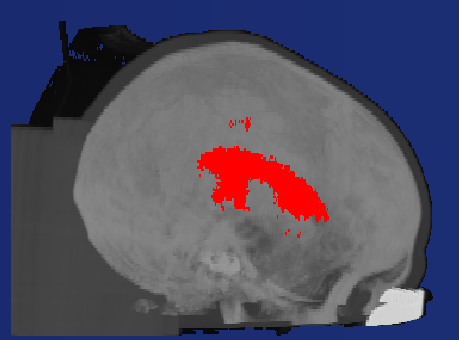
\includegraphics[width=\textwidth]{Logos/Normal1/Seite.PNG}
\captionof{figure}{Visualisierung des ersten normalen Ventrikelsystems von der Seite}
\label{fig:norm1_s}
\end{minipage}
\begin{minipage}[c]{0.49\textwidth}

\includegraphics[width=\textwidth]{Logos/Normal1/Unten.PNG}
\captionof{figure}{Visualisierung des ersten normalen Ventrikelsystems von Unten}
\label{fig:norm1_s}
\end{minipage}



\todo{SATZBAU!!!}
Das Verfahren wurde an 15 verschiedenen CT-Daten getestet. Darunter waren Ventrikelsysteme, von denen vier normal, vier schlank, zwei unter Atrophie leidend, zwei mit einem Mittellinienshift, eins deformiert, eins Blutresorbiertes und eins Hydrocephalus waren.
\newline
Die normalen und die schlanken Ventrikelsysteme benötigen keiner weiteren Erklärung. Bei den Normalen glückte die Visualisierung bei zwei Stück. Die Schlanken, waren leider für das Verfahren nicht zu erfassen, weshalb es davon keine zufriedenstellende Visualisierung gibt. Atrophie bezeichnet den, oft durch das Alter verursachten, Schwund von Hirnmasse. Hierbei war es bei einem der beiden Datensätze möglich das Ventrikelsystem sichtbar zu machen. Bei dem Mittellinienshift, der Verschiebung der Mittellinie des Ventrikelsystems, dem Deformierten, dem Blutresorbiertem und dem Hydrocephalus, einer Aufstauung von Nervenwasser im Kopf, war aus jeweils dem Grund der Unterschiede der Daten zum normalen Ventrikelsystem mit dem aktuellen Stand der Implementierung keine erfolgreiche Visualisierung möglich.
\newline
Für die erfolgreich visualisierten Daten wurde zur Evaluation ein Arzt von der Uniklinik Ulm befragt. Diesem wurden die Visualisierungen drei verschiedener Ventrikel vorgeführt, zwei normale Ventrikel und ein Ventrikel mit Atrophie. Screenshots der Visualisierung des 2ten normalen und des atrophie Venktrikels sind im Anhang zu sehen. Der erste normale Ventrikel, ist in \autoref{fig:ventrikel_seite, fig:ventrikel_unten, fig:ventrikel_oben} zu sehen. Während der Vorführung konnte der Mediziner selbst die Kamera durch die Darstellung lenken. Anschließend bewertete er, mit der Beantwortung von drei verschiedenen Fragen auf einer Skala von eins bis fünf, die Qualität der Ergebnisse.
\begin{itemize}
	\item 1) Wie gut ist das Ventrikelsystem bei der Visualisierung zu erkennen? \newline sehr schlecht 1 - 5 sehr gut
	\item 2) Wird das Ventrikelsystem in der Visualisierung vollständig dargestellt? \newline überhaupt nicht vollständig 1 - 5 vollständig
	\item 3) Wie genau ist das Ventrikelsystem segmentiert? \newline überhaupt nicht segmentiert 1 - 5 ausschließlich das Ventrikelsystem ist segmentiert
\end{itemize}


Die Ergebnisse zu den verschiedenen Visualisierungen werden in \autoref{tab:ergebnis_arzt} gezeigt.

\begin{table}[h]
\centering
\resizebox{\columnwidth}{!}{
 \begin{tabular}{| c | c | c | c |}
  \hline
  Ventrikelsystem & 1. Frage & 2.Frage & 3. Frage\\ \hline
  Normal 1 & 4 & 4 & 3 \\ \hline
  Normal 2 & 4 & 2 & 3\\ \hline
  Atrophie & 4 & 3 & 2 \\ \hline
 \end{tabular}
 }
\caption{Ergebnisse des Interviews mit einem Arzt}
\label{tab:ergebnis_arzt}
\end{table}



Der Arzt merkte an, dass bei jeder Visualisierung, die durch das Verfahren erzeugt wurde, nur der linke und rechte Seitenventrikel zu sehen war. Die deutlich schmaleren dritten und vierten Ventrikel und die Unterhörner der Seitenventrikel fehlten bei den Darstellungen komplett. Diese sind bei einem gesunden Menschen jedoch klein und deshalb schwer zu segmentieren. Weiterhin sind diese Teile für die Ventrikelpunktion ohnehin uninteressant, da die Punktion im Vorderhorn eines Seitenventrikel stattfindet, also einem Bereich den die Visualisierung abdeckt. Folglich sind die Antworten auf die zweite Frage, nach der Vollständigkeit des Ventrikelsystems, lediglich Vollständigkeit der beiden Seitenventrikel zu sehen.
\newline
Die Bewertung des ersten normalen Ventrikelsystems fiel positiv mit 11 von möglichen 15 Punkten aus. Das Ventrikelsystem war als solches klar zu erkennen, jedoch fehlten die Hinterhörner ein wenig. Bis auf diese waren die Seitenventrikel auch vollständig zu sehen. Bei der Segmentierung gab es mehrere kleine Ausreißer.
\newline
Der zweite normale Ventrikelsystem, war auch gut zu erkennen. Jedoch wird fast ausschließlich der linke Seitenventrikel visualisiert, weshalb die 4 als Bewertung auf diesen bezogen war. Dieser ist dafür jedoch sehr klar, deutlich und vollständig zu sehen. Der Arzt sagte, dass dieser besser und glatter als die des ersten normalen Ventrikelsystems sein, da man auch das Unterhorn erkennen kann. 
\newline
Bei einer Atrophie ist im Gehirn deutlich mehr Liquor zu finden als bei einem gesunden. Diese werden vom Verfahren auch erkannt, weshalb die Segmentierung etwas verschwimmt und nicht die kompletten Seitenventrikel erfasst werden. Jedoch ist zu vermuten, dass viele der Ausreißer zum dritten Ventrikel gehören, da dieses, wie alle Ventrikel bei einer Atrophie sich weitet. Trotz der Flüssigkeiten im Gehirn war das Ventrikelsystem in der Darstellung gut zu erkennen.
\newline
 Im Allgemeinen sagte der Mediziner, dass das Ventrikelsystem als solchen ganz eindeutig zu erkennen sei, allerdings sei die Darstellung nicht glatt genug.


\begin{minipage}[c]{0.49\textwidth}
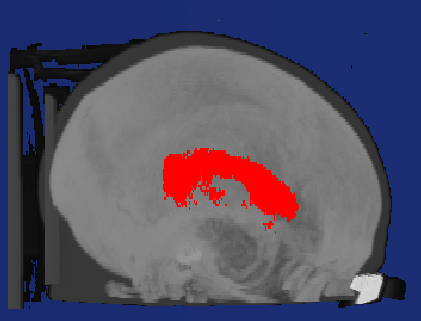
\includegraphics[width=\textwidth]{Logos/Normal2/Seite.PNG}
\captionof{figure}{Visualisierung des zweiten normalen Ventrikelsystems von der Seite}
\label{fig:norm2_s}
\end{minipage}
\begin{minipage}[c]{0.49\textwidth}

\includegraphics[width=\textwidth]{Logos/Normal2/Unten.PNG}
\captionof{figure}{Visualisierung des zweiten normalen Ventrikelsystems von Unten}
\label{fig:norm2_u}
\end{minipage}



\begin{minipage}[c]{0.49\textwidth}
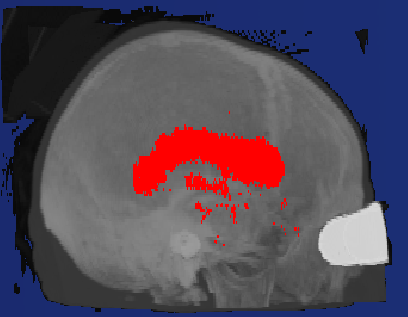
\includegraphics[width=\textwidth]{Logos/Atrophie/Seite.PNG}
\captionof{figure}{Visualisierung des Atrophie Ventrikelsystems von der Seite}
\label{fig:atro_s}
\end{minipage}
\begin{minipage}[c]{0.49\textwidth}

\includegraphics[width=\textwidth]{Logos/Atrophie/Unten.PNG}
\captionof{figure}{Visualisierung des Atrophie Ventrikelsystems von Unten}
\label{fig:atro_s}
\end{minipage}




Zum weiteren Vergleich der Ergebnisse wurde das erste normale Ventrikelsystem in Unity und mit der MITK-Workbench, die auch zum Umwandeln der DICOM-Dateien benutzt wurde, visualisiert.
\newline
In Unity wurde dabei die Erweiterung zum hervorheben von Wertebereichen benutzt. Diese wurde auf 1025 bis 1030 eingestellt, da das Ventrikelsystem Intensitätswerte in diesem Bereich hat. Die Ergebnisse sind in \autoref{fig:unity_s} und \autoref{fig:unity_u} zu sehen.
\newline
Das Ventrikelsystem ist zwar zu sehen, es gibt jedoch sehr viele Ausreißer, die es fast unmöglich machen die Ventrikel zu erkennen. Diese simple Vorgehensweise führt zu keinem gewünschtem Ergebnis.
\newline
In der MITK-Workbench gibt es verschiedene Segmentierungstools. Darunter ist ein Region Growing Tool, bei dem der Nutzer einen \textit{seed} Punkt in den Schnittbildern wählen kann. Über die verwendete Kostenfunktion werden keine Informationen genannt. Anschließend können die Löcher der Auswahl mit einem \textit{closing} Filter geschlossen und mit einem weiteren Tool ein geglättete 3D Ansicht des Ergebnis erzeugt werden. Screenshots des Ergebnisses sind in \autoref{fig:mitk_o} und \autoref{fig:mitk_v} zu sehen.
\newline
In dem von der Workbench erzeugte Ergebnis ist das Ventrikelsystem gut zu erkennen. Die Seitenventrikel sind vollständig und besitzen eine glatte Oberfläche. Sogar große Teile des dritten und vierten Ventrikels sind teil der Segmentierung.



\begin{minipage}[c]{0.49\textwidth}
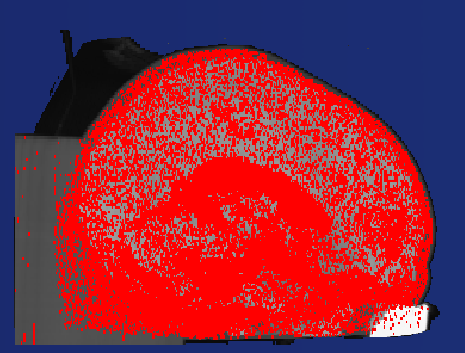
\includegraphics[width=\textwidth]{Logos/Normal1_Unity/Seite.PNG}
\captionof{figure}{Visualisierung des ersten normalen Ventrikelsystems von der Seite mithilfe von Unity}
\label{fig:unity_s}
\end{minipage}
\begin{minipage}[c]{0.49\textwidth}

\includegraphics[width=\textwidth]{Logos/Normal1_Unity/Unten.PNG}
\captionof{figure}{Visualisierung des zweiten normalen Ventrikelsystems von Unten mithilfe von Unity}
\label{fig:unity_u}
\end{minipage}


\begin{minipage}[c]{0.49\textwidth}

\includegraphics[width=\textwidth]{Logos/Normal1_MITK/Oben.PNG}
\captionof{figure}{Visualisierung des ersten normalen Ventrikelsystems von Oben mithilfe von MITK}
\label{fig:mitk_o}
\end{minipage}
\begin{minipage}[c]{0.49\textwidth}
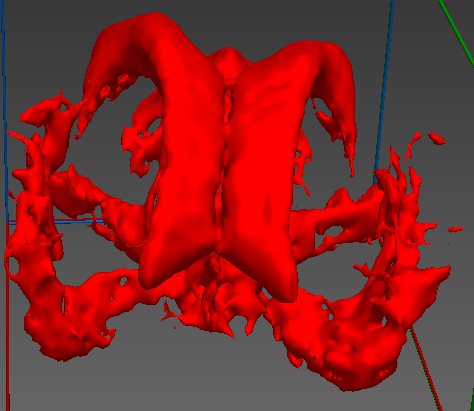
\includegraphics[width=\textwidth]{Logos/Normal1_MITK/Schraeg_Vorne.PNG}
\captionof{figure}{Visualisierung des ersten normalen Ventrikelsystems von Vorne mithilfe von MITK}
\label{fig:mitk_v}
\end{minipage}





\todo{nutzerstudie variablen etc. erwähnen -> proseminar}
\todo{info über teilnehmer}
Im Rahmen der Evaluation der Benutzerfreundlichkeit des Verfahrens wurde eine kleine Nutzerstudie mit ... Teilnehmern durchgeführt. Bei dieser wurden den Probanden zunächst der Ablauf und die vom Benutzer erforderlichen Schritte um eine Visualisierung des Ventrikelsystems zu erhalten durch eine Vorführung durch den Interviewer gezeigt. Anschließend mussten die Teilnehmer selbst das eben gelernte anwenden und das Programm selber ausführen. Dabei bekamen sie, wenn sie nicht weiterwussten, Hilfe vom Versuchsleiter. Als Abschluss füllten die Probanden einen NASA-TLX Bogen zu der Aufgabe aus. Die durchschnittlichen Ergebnisse der einzelnen Kategorien wird in \autoref{tab:ergebnis_nasa} gezeigt.


\begin{table}[h]
\centering
\resizebox{\columnwidth}{!}{
 \begin{tabular}{| c | c | c | c |}
  \hline
  Kategorie & Gewichtung & Klicks & Wichtung \\ \hline
  Geistige Anforderung & 0&0 &0 \\ \hline
  Körperliche Anforderung & 0& 0& 0\\ \hline
  Zeitliche Anforderung &0 &0 &0 \\ \hline
  Leistung &0 &0 & 0\\ \hline
  Anstrengung &0 & 0& 0\\ \hline
  Frustration &0 &0 & 0\\ \hline 
 \end{tabular}
 }
\caption{Durchschnittlichen Ergebnisse des NASA-TLX Bogens}
\label{tab:ergebnis_nasa}
\end{table}


Der durchschnittliche Wert für die Gesamtbeanspruchung lag bei ... Personen ohne Programmiererfahrung ...

 
Trotz der Schwierigkeiten,  gaben die Probanden an, dass sie die Aufgabe mit einer guten ausführlichen Dokumentation auch alleine ohne Hilfe hinbekommen würden.



Die folgenden Zeitmessungen wurde alle auf einem Computer mit einem 3.70GHz  Intel Core(TM) i7-8700K CPU mit 32GB RAM ausgeführt.
\newline
Um die Berechnungszeit des Systems messen zu können, wurde die Berechnung des gesamten Clusteringverfahrens und die des LH-Histogramms mit drei verschieden großen Volumen durchgeführt. Diese stammen alle von den gleichen CT-Daten ab und wurden lediglich  mit dem Resamplemodul auf die Hälfte beziehungsweise Dreiviertel der ursprünglichen Größe verkleinert. Es war geplant, dass noch ein viertes Volumen zum Vergleich hinzugezogen wird, jedoch war es aus einem unbekannten Fehler leider nicht möglich die Verfahren mit einem gevierteltes Volumen durchzuführen. Desweiteren funktioniert bem ganzen Volumen lediglich die Berechnung des LH-Histogramms, die komplette Verfahren ist nicht möglich, vermutlich aus dem Grund, dass es zu viele Daten für die aktuelle Implementierung sind.
\newline
Die Berechnungszeit hängt stark von der Größe des Eingabevolumens ab. Die ist in \autoref{tab:ueberblick_zeit} sehr gut zu erkennen. Diese zeigt einen Überblick über die ungefähren Berechnungszeiten der verschiedenen Volumengrößen.


\begin{table}[h]
\centering
\resizebox{\columnwidth}{!}{
 \begin{tabular}{| c | c | c | c |}
  \hline
  Volumengröße & LH-Histogramm $[s]$ & Komplettes Verfahren $[s]$ \\ \hline
  Halbes Volumen (256x101x256)  & 30 &  50	\\ \hline
  Dreiviertel Volumen (384x151x384)  & 90 &  380	\\ \hline
  Ganzes Volumen (512x201x512) & 225 & -	\\ \hline
 \end{tabular}
 }
\caption{Überblick über die Berechnungszeiten der verschiedenen Volumengrößen}
\label{tab:ueberblick_zeit}
\end{table}


Dabei ist wichtig zu beachten, dass die Zeit zur Berechnung der LH-Histogramme die gleiche Zeit wie die Berechnung der LH-Werte im gesamten Verfahren benötigt. Die Berechnungsdauer der Gradienten ist hierbei zirka doppelt so lange wie die der LH-Werte. Zieht man die Berechnungszeit des Histogramms von der Kalkulationszeit des gesamten Verfahrens ab, erhält man die Zeit, die die beiden Clusteringschritte benötigen.
\newline
Eine interessante Beobachtung hierbei ist, dass die Berechnung der LH-Histogramme abhängig von der Anzahl der Pixel gesehen in etwa gleich schnell abläuft. Das halbe Volumen hat eine Gesamtpixelzahl von ungefähr 6,6 Millionen, das dreiviertel Volumen von zirka 22,2 Millionen und das ganze Volumen von grob 52,6 Millionen Pixeln. Wird die Anzahl an Pixeln die pro Sekunde bei der LH-Wert Berechnung bearbeitet werden für diese drei Volumen berechnet, so ist zu beobachten, dass keine großen Unterschied zwischen den Zeiten existiert. Das Halbe bearbeitet etwa 220 Tausend, das Dreiviertel ungefähr 247 Tausend und das Ganze 234 Tausend Pixel pro Sekunde. Der kleine Unterschied in der Rate lässt sich einerseits durch feste Berechnungen, die unabhängig von der Pixelzahl sind, und andererseits über nicht ganz genauen Messungen erklären. Folglich kann man sagen, dass die Berechnungszeit der LH-Werte bei dieser Implementierung in etwa linear mit der Anzahl an Eingabepixeln wächst.
\newline
Auf der anderen Seite ist jedoch auch zu erkennen, dass die beiden Clusteringschritte mit zunehmender Eingabegröße deutlich langsamer werden. Das Clustering des halben Volumens dauerte 20 Sekunden und hat damit eine Verarbeitungsrate von zirka 330 Tausend Pixeln pro Sekunde. Hingegen dauert es beim dreiviertel Volumen 290 Sekunden und erreicht damit gerade einmal einen Rate von 76 Tausend Pixeln pro Sekunde. Es braucht also 14,5 mal so lange an Zeit für die 3,3 fache Anzahl an Pixeln.














































